%!TEX root = ../thesis.tex
\chapter{Results}
\label{chap:Results}
In this Chapter I present the results of applying the methodology explained in Chapter \ref{chap:BHM} to the Pleiades DANCe data set (Sect \ref{sect:PleiadesDANCe}). However, to characterise the methodology and estimate its precision and accuracy, I first apply it over synthetic data. Using this data, I am able to analyse the performance of the methodology when it is considered only as a classifier. Later, in this Chapetr I give the results of our methodology main objective: the statistical characterisation of the cluster population. In the following Sections I give the details of the spatial, velocity, luminosity and mass distributions. Later, I will describe the physical scenario of the evolution of the mass distribution by comparing the Pleiades mass distribution with other younger and older clusters. Finally, I will end this Chapter with a description of how the Bayesian methodology allowed us to update our previous knowledge of the Pleiades cluster.

\section{Performance of the classifier}
\label{classifier}
As mentioned earlier, the main objective of our the methodology of the BHM is the statistical characterisation of the NYOC populations. As a by product, it also obtains individual membership probability distributions. Using these last ones, we are able to directly classify objects into cluster and field members, providing that and objective probability threshold has been stablished. The objective of this section is to find this objective threshold by means of synthetic data. As any other measured property, this classification has an uncertainty, thus, the purpose of this section is also to quantify this uncertainty. 

That said, in order to properly characterise our classifier, I test it over synthetic data sets that resemble the real data. An ideal test to our classifier will be to apply it over well known dataset in which tags of cluster and field members were already present. However, if we may have access to these tags, a classifier may not be needed. The Pleiades cluster being \emph{the} most studied cluster in history, is the  NYOC with most of these tags. This is the reason for which we decided to benchmark our methodology on it. Nevertheless, the problem of the synthetic data remains since the low-mass end of the cluster still is \emph{terra ignota}. To over come this issue, we decided to create synthetic data sets under the assumption that our cluster and field models resemble the real data.  We are aware that these models are far from perfect, but so far is the best we can do. 

The assumption that our model correctly models the real data, although enable us to measure the uncertainty of our classifiers, does not give any indication about possible biases in our model. To explore this possibility, we later compare our real data results with those found in the literature. I present this comparison at the end of this section.

Hence, we fit our models, field and cluster, to the real data ($10^4$) and using the MAP estimates, we created synthetic stars (five samples of $10^4$ objects each). To further test the reliability of our classifier, we compare the results it render when applied over data sets with and without missing values. This comparison allows us to quantify the impact that missing values have on our results.    

One further consideration. The synthetic analysis requires at least three runs: one on the real data to obtain the MAP, and two on the synthetic one: with and without missing values. However, as explained in Chapter \ref{chap:BHM}, our methodology is computationally expensive. Therefore, to maintain the computing time within reasonable limits (couple of weeks), we decided to restrict our synthetic data set to only the $10^4$ objects with higher membership probability according to \citet{Bouy2015}. I elaborate on the consequences of this decision.

These $10^4$ objects are "closer" to the cluster in the sense of membership probability than the remaining 9$\times 10^4$ objects. Therefore, the field probability density rendered by this sample, compared to that of the larger $10^5$ sample, has the following properties: it is more concentrated and has larger values near the cluster region. Since the $10^5$ sample is largely dominated by the field population, its density peaks far form the cluster proper motion and photometric sequences. Densities are normalised, thus more of the density mass of this large sample is far from the cluster region. 

Given the previous considerations, we assume that results obtained on the smaller $10^4$ sample have are more contaminated, and have lower recovery rates than those obtained on the larger and more distant $10^5$ sample. On the one hand, the higher contamination rate results from the larger concentration of the field density around the cluster region.  On the other hand, the lower recovery rates arises from the higher values of the field probability density. In simple words, when we define the field in a more restricted region around the cluster, both populations become more entangled, thus they become more difficult to separate. Therefore, we assume that the results obtained on the smaller $10^4$ sample represent upper and lower limits to the contamination and recovery rates of the larger $10^5$ sample, respectively.

Briefly, to create the synthetic data set, the procedure is the following. First, using the methodology of the previous Chapter, I obtain a sample of the posterior distribution of the parameters given the $10^4$ real data set. Then, I chose the particle with highest posterior probability as the MAP estimate of the posterior distribution. Using this particle positions I generate five synthetic data sets of $10^4$ objects each. Then, I tag these objects according to their parent population: cluster or field. Then, using the synthetically observed values I estimate their uncertainties and missing value patterns (more details  below). Finally, I run the model over these five synthetic samples and compare the measured tags with the true ones as function of the probability threshold.

 Also, I run the methodology over the synthetic data set without missing values and compare this results with those found on the same data set with missing values. This test, as mentioned before, enable us to quantify the impact of missing values over individual membership probabilities.  

As explained in Sect. \ref{sect:pleiadesdataset}, our data set has a high fraction of missing values. Only $\sim1\%$ has completely observed entries. Furthermore, the missing pattern is not random and depends on the magnitudes and colours of the objects. Therefore, to better reproduce this pattern, for each synthetic datum, we use missing value template of one of its closer neighbours in the real data; closer in the euclidean sense. Using the missing value template of the nearest neighbour from the real data set results in a biased sample in which objects with complete (non missing) values are underestimated. This is the inevitable consequence of the fact that euclidean distances measured in subspaces resulting from the missing values, are smaller or, at most, equal to those measured in the non-missing value spaces. 

Missing values are assigned as follows. Since by definition of our data set there are no missing values in our proper motion data, missing values were assigned only to photometry. We chose the closer neighbours from the available CMDs: $\{K_s,J-K_s\},\{J,J-H\},\{K_s,H-K_s\},\{J,Y-J\},\{K_s,i-K_s\}$. These CMD are formed with the bands and colours with fewer missing values, in decreasing order.  The missing value pattern for individual objects was chosen as follows. First, for each CMD subspace we find the fraction, $f_r$, of objects from real data without missing values, we call it $C_{or,i}$. Then, we take a random sample from the synthetic data whose fraction, $f_s$ corresponds to $f_r$. For objects in this sample we assign the missing value pattern of the nearest neighbour from sample $C_{or,i}$. We repeat the procedure for all CMDs. In this way, the synthetic data has fractions of missing and non-missing values similar to those of the real data.

Uncertainties are assigned as follows. We set the proper motions uncertainties to those of the nearest neighbour in the real data. IN photometry, however, this scheme renders uncertainties that are biased towards the less precise measurements. This is a consequence of the missing values. Again, the euclidean metric results in the preferential choosing of objects with missing values. These missing values occur mostly at the faint end, where uncertainties are larger. Therefore, the uncertainties are biased towards larger values. To avoid this issue, we fit polynomials (8th degree) to the uncertainties as a function of the magnitudes. Then, we use these polynomials to give uncertainties to the synthetic photometric data.

The performance of our classifier was measured by counting the true positives (TP, cluster members correctly classified), true negatives (TN, field members correctly classified), false positives (FP, field members classified as cluster members) and false negatives (FN, cluster members classified as field members) recoveries as a function of the probability threshold. With them we calculate the true positive rate, contamination rate, accuracy and precision, which are defined as follows. In order to classify the objects as cluster of field members we summarise their membership probability distribution using the mode. If the mode is grater than the current probability threshold, then the object is classified as cluster member, if not as field.

The true positive rate (TPR) is the ratio of true positives over the sum of true positives plus false negatives. The contamination rate (CR) is the ratio of false positives over the sum of false positives plus true positives. The precision or positive predictive value (PPV) is the ratio of true positives over the sum of true positives plus false positives. Finally, the accuracy (ACC) is the ratio of the sum of true positives plus true negative over the sum of true and false positives and negatives. These are,

\begin{align}
TPR &= \frac{TP}{TP+FN} \nonumber \\
CR   &= \frac{FP}{FP+TP} \nonumber \\
PPV &= \frac{TP}{TP+FP} \nonumber \\
ACC &= \frac{TP+TN}{TN+FN+TP+FP} \nonumber
\end{align}

We use the results of the five synthetic data sets to quantify the uncertainties of the previous quantities. 

In Fig. \ref{figure:tfpr} I show the TPR and CR, as a function of probability threshold, computed for the cases in which missing values where both present and absent. The missing value case was computed for the five synthetic samples, thus, the lines and the shaded grey regions depict the mean and maximal deviations, of the results found on the five synthetic samples. As can be seen in this Figure, the missing values have a negative impact in our classification. They cause a diminishing of the TPR  and an increase in the CR. This negative impact is expected since the observables we are using are highly discriminant in the classification process. Since cluster and field are highly entangled in our $10^4$ synthetic samples, when a highly discriminant observable is missing the classification process could be biased or more uncertain.

In spite of the negative impact of missing values, our methodology delivers low ($\lesssim 8\%$) contamination rates and high recovery rates. In Figure \ref{figure:tfpr} we also show , for the sake of comparison, the CR and TPR of \citet{Sarro2014} (reported in their Table 4). 

From the previous comparison we observe that the TPR delivered by of our methodology: i) when measured on data without missing values, is similar to that of \citet{Sarro2014} methodology. This is expected since the results of those authors are based on a model constructed only with completely observed objects (i.e. non-missing values). ii) when measured on data with missing values, is $\approx 4\%$ lower than that of \citet{Sarro2014}. 

This last figure is a small price to pay compared to the dramatical increase in the number of sources used to construct our model (both field and cluster). As mentioned in Section \ref{sect:pleiadesdataset}, in our $10^5$ objects data set, only $\sim 1\%$ of objects have completely observed entries. Roughly, this is the fraction of sources used by \citet{Sarro2014} and \citet{Bouy2015} to construct their models. 

On the other hand, the CR of our methodology, above $p=0.8$ and for both missing-values and non-missing values cases, outperform, by $x\%$, the CR reported of \citet{Sarro2014} methodology, see below.

In simple words, what can be observed from the previous analysis is that our methodology, compared to that of \citet{Sarro2014}, renders less contaminated (CR) results ($x\%$) at the price of a smaller recovery rate (TPR) $4\%$

Nonetheless, we stress the fact that the previous comparison is not straight forward. The following reasons must be born in mind. First, \citet{Sarro2014} infer their cluster model using only non-missing-value objects, later they apply that model to objects with and without missing values. Second, their synthetic data set and ours are essentially different. They are constructed with different generative models, different number of elements, and different missing value patterns. 

Now, I describe the procedure to set an objective probability threshold. This probability threshold, although is not needed to obtain the distribution of the cluster population, is needed however to objectively classify an object. Since real data contain missing values, there is no need establish this threshold for the non-missing values case. There are different approaches to establish this probability threshold, however I only use the approach of maximum accuracy (ACC). 

Figure \ref{figure:tfpr} shows the ACC and the PPV of our classifier when applied on synthetic data with missing values. The lines and the grey regions depict, respectively, the mean and the maximum deviations of the five synthetic data set results. We use these last ones as the uncertainty of our estimates. The mean of the highest accuracy, ACC=$96.5\pm0.1$\%, happens at probability threshold $p_t = 0.84$. At this threshold the CR is $4.3\pm0.2$\%, the TPR is $90.0\pm0.05$\%, the ACC is , and the PPV is $95.6\pm0.2$\%. 

\begin{figure*}[!htp]
\begin{center}
%\resizebox{\hsize}{!}{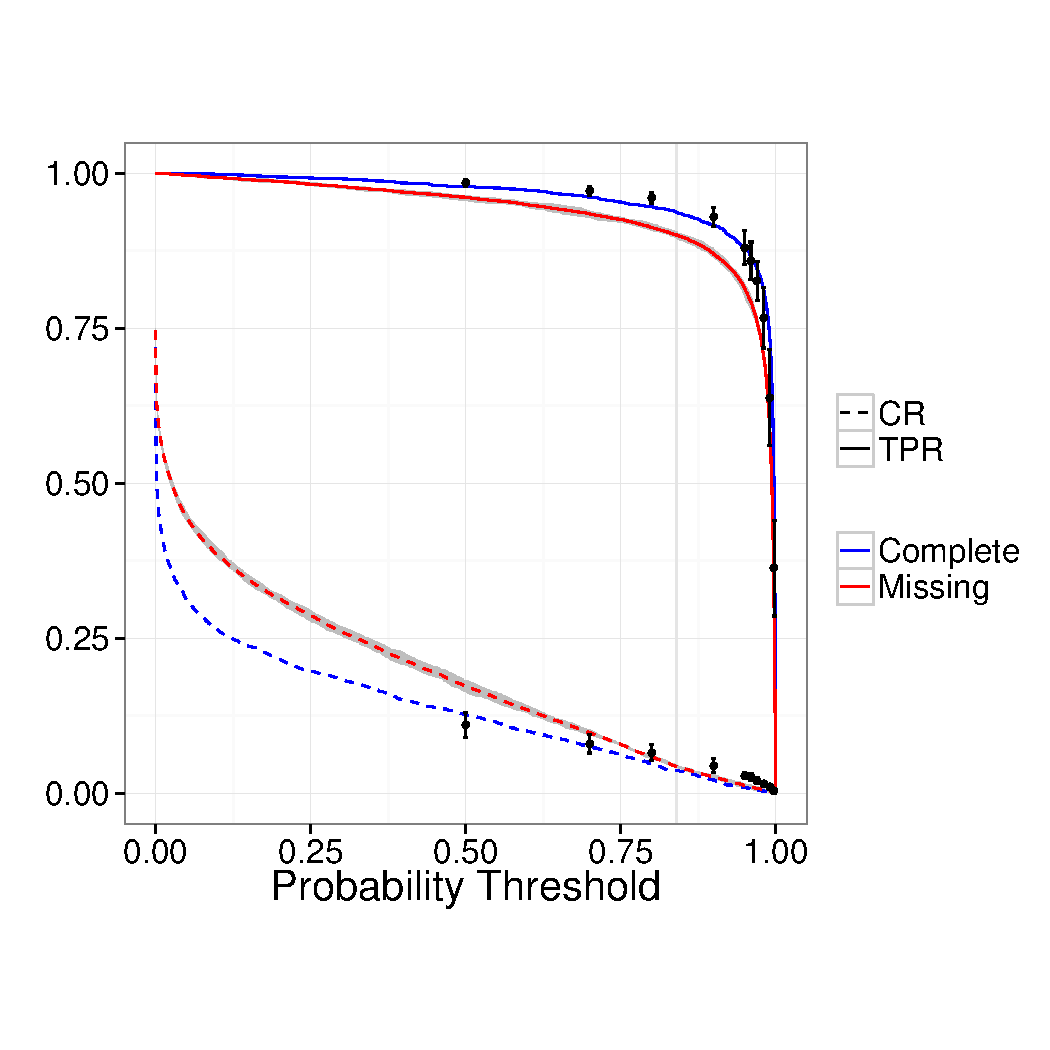
\includegraphics{figs/FTPRvsSarro.pdf}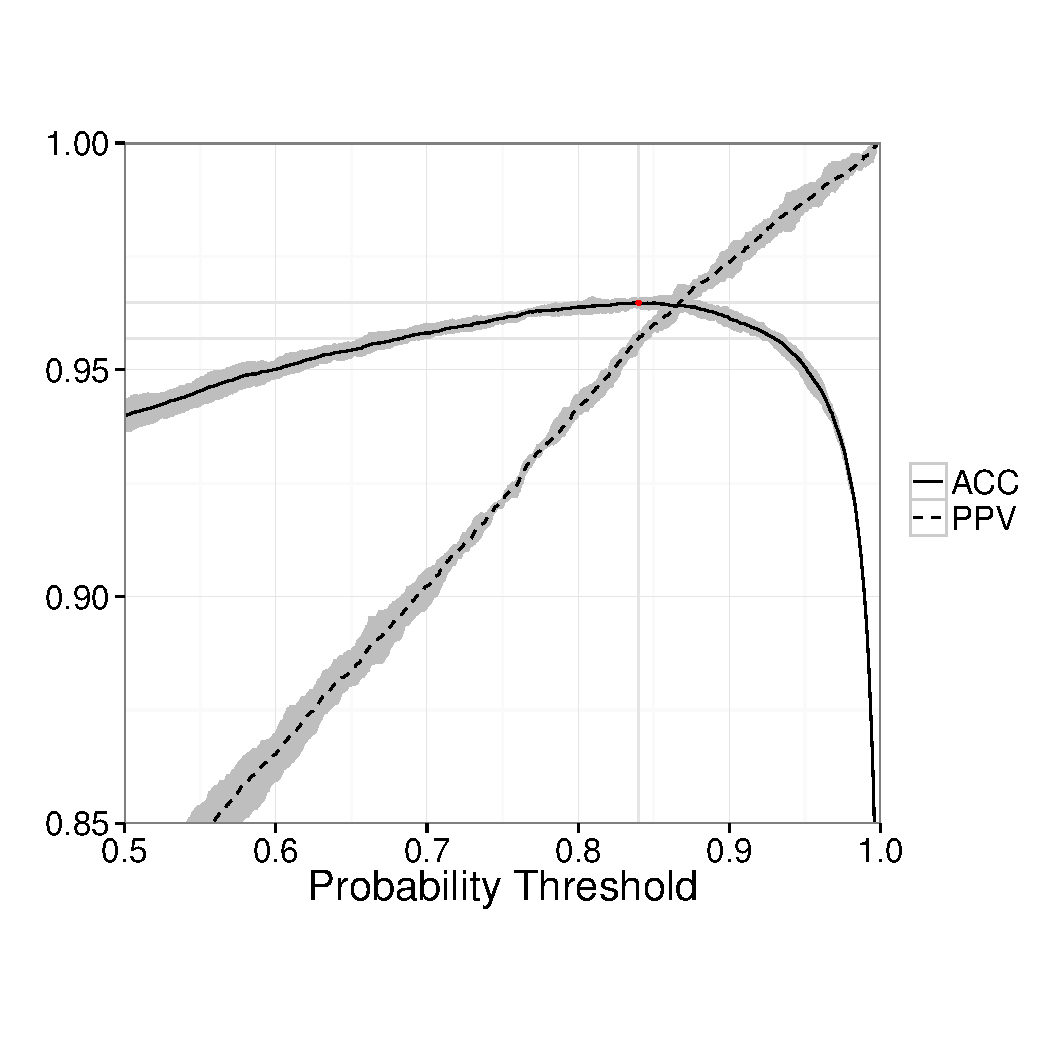
\includegraphics{figs/PrecisionAccuracy.pdf}}
\caption{Left: The TPR (solid line) and CR (dashed line) of our methodology  when applied on synthetic data sets with and without missing values (red and blue lines, respectively). In black dots we show the TPR and CR reported by \citet{Sarro2014} for their non-missing values model. Right: Accuracy and precision as a function of probability threshold for our classifier when applied on synthetic data with missing values. The higher accuracy is obtained at $p_t=0.84$ (red dot). In both panels, the grey areas show the maximum deviations from the mean of the results of the five missing-values synthetic data sets.}
\label{figure:tfpr}
\end{center}
\end{figure*}

We investigate further on the impact of missing values, particularly to analyse any possible biases introduced by them. It was done by comparing the mode of the individual membership probability distributions found after fitting the model to data sets with and without missing values. The missing values data set is the result of adding a mask of missing values (as previously described) to the completely observed data set. It means that this data set has identical observed values, except for those masked as missing ones. 

In Fig. \ref{figure:IncVsCom} we show the mode of the membership probabilities of objects with missing values (vertical axis) against those of non-missing values (horizontal axis). As can be seen in this Fig., the missing values impact our results by spreading the membership probabilities. Ideally, we would like to recover membership probabilities following the line of slope one, as in the case of completely observed values (red squares). The most striking deviations come from objects lacking the $CI$ (enclosed in black). Our methodology uses the \emph{true} $CI$ to prescribe the \emph{true} photometry, and the observed $CI$ to constrain the marginalisation integral of the \emph{true} $CI$. Thus, it is expected that a missing $CI$ will produce a probability spread. These missing $CI$ objects show two different behaviours. In one case, there are sources with membership probabilities $p_{complete} \approx0$ which have overestimated probabilities in the incomplete case (vertical axis). In the other case, the sources in the combed area below the line of unit slope have underestimated probabilities in the incomplete case. While the first case contributes to the CR the second one diminishes the TPR. The first case reaches the maximum difference at $p \approx 0$ (difference between red and blue dashed lines in Fig. \ref{figure:tfpr}), thus its impact in our results is marginal. Furthermore, at our objective probability threshold $p_t=0.84$, these objects have a small impact in our results, they represent only 1.8\% of the contamination rate. The box region in Fig. \ref{figure:IncVsCom} shows them. The second case, however, typify the unavoidable loss of members due to the missing values, 4\% at $p_t=0.84$, given our model and the observables it uses.


The bias introduced by missing values can be estimated using the root-mean-square (rms) of the difference between membership probabilities recovered with and without missing values. The total rms is 0.12. On the one hand, objects with completely observed values (red squares) in both data sets have a rms of only 0.02. On the other hand, objects with missing values have a rms of X. While the rms of objects lacking the $CI$ have and rms of .  The previous effects show an overall agreement between results on data sets with and without the missing values, nonetheless, care must be taken when dealing individually with objects lacking the $CI$. 


As mentioned before, our methodology aims at the statistical distributions of the cluster population. It works by ensuring that each object contributes to the cluster distributions proportionally to its cluster membership probability. In this sense our results are free of any possible bias introduced by hard cuts in the membership probability. Nevertheless, contamination is still present and must be quantified. To quantify it, I compute the expected value of the CR. It is $\langle CR \rangle=5.8\pm 0.2$\%. In this expected value, each CR contributes proportionally to the  probability threshold at which it is measured. 

\begin{figure}[!htp]
\begin{center}
%\resizebox{\hsize}{!}{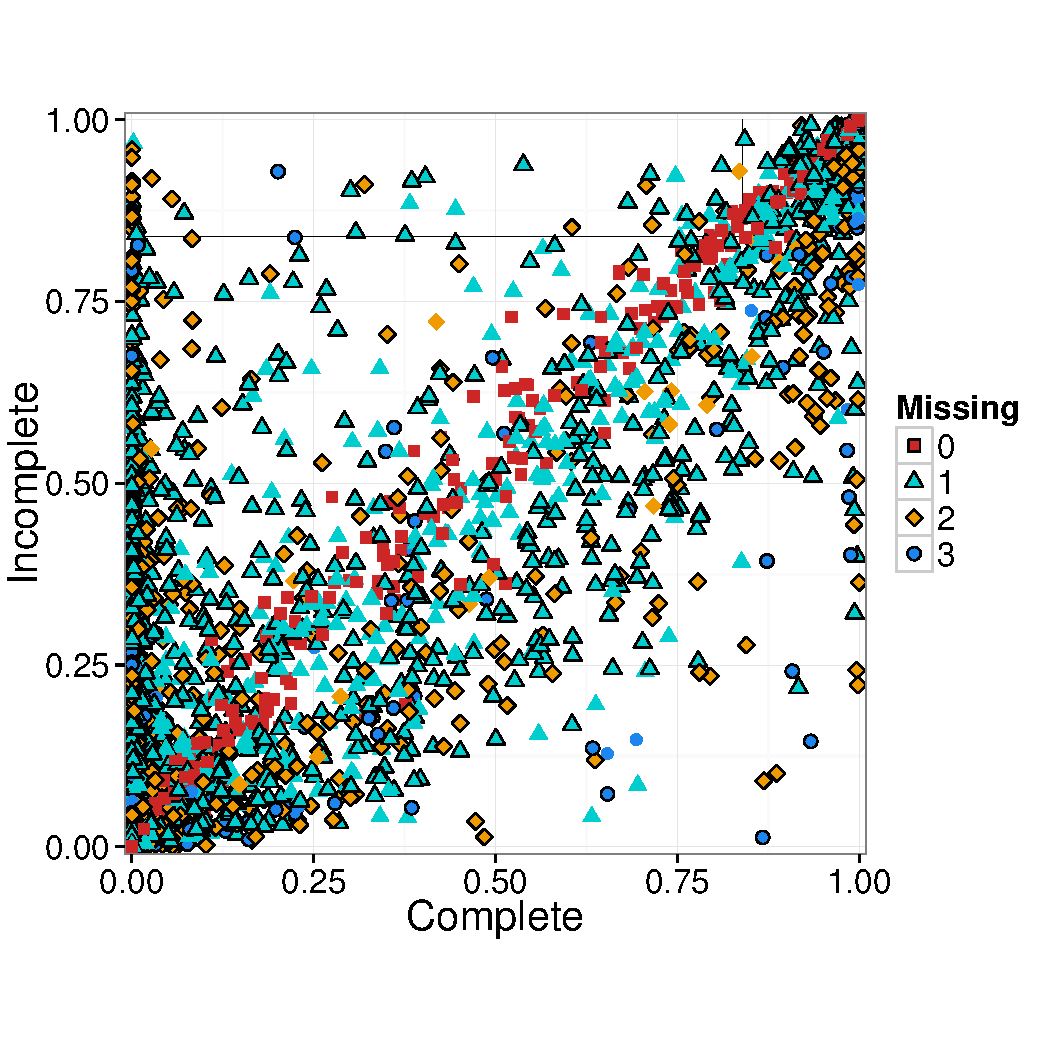
\includegraphics[page=1]{figs/Probabilities.pdf}}
\caption{Comparison between the cluster membership probabilities recovered from the synthetic data with missing values (Incomplete) and without them (Complete). The colour and shape indicate the amount of missing values. The symbols enclosed in black indicate a missing $CI$. The top left box contains objects considered as contaminants due to missing values, at the probability threshold $p_t=0.84$.}
\label{figure:IncVsCom}
\end{center}
\end{figure}
 
\subsection{Comparison with the literature}
In Section \ref{sect:pleiades} I mentioned that the most important works on the Pleiades members are those of \citet{Stauffer2007,Lodieu2012,Sarro2014,Bouy2015}. In this section I will compare the list of candidate members found in this work using the probability threshold found in the previous section with those of the most recent study, the one from \citet{Bouy2015}. Later I will broadly compare my list of candidate members with the one of \ref{Stauffer2007}. 
\subsubsection{Candidate members from \citet{Bouy2015}}
The methodology of this work, although essentially different from that of \citet{Bouy2015}, the fact that both share the data set and use the same observables, allows a direct comparison between them. When using their objective probability thresholds, as shown by Fig. \ref{figure:HM-SBB}, both methodologies agree on the outstanding $99.6$\% of the classified objects. Concerning the candidate members, they also agree on $\approx 90\%$ of them. Nevertheless, the discrepancies are worthy of discussion.

The rejected candidates of \citet{Bouy2015} (lower right box of Fig. \ref{figure:HM-SBB}) amount to 12\% of their total number of candidate members. This value is 4.7\% higher than the contamination rate reported by \citet{Sarro2014}: $7.3\pm1.4$\%. I will not reject a priori these objects as candidate members because, as mentioned in Sect. \ref{sect:classifier}, our methodology recovers 4\% less members when compared to that of \citet{Sarro2014}(see Fig. \ref{fig:tfpr}). The majority, $85\%$, of these objects have missing values, which indicates that these objects require future follow up. Even the 37 completely observed and rejected candidates can not be discarded as true members due to the fact that our methodology losses 6\% of the true cluster members (see Fig. \ref{fig:tfpr}).  

On the other hand, our new candidates (upper left box of Fig. \ref{figure:HM-SBB} ) amount to 10\% of \citet{Bouy2015} candidates. This figure is higher than the $4.3\pm0.2$\% CR reported on the previous Section. Thus, it indicates that up to $\sim6\%$ of these objects can be true cluster members. From these objects, one half have completely observed values, thus 3\% of our new candidates are completely observed objects. This las figure agrees perfectly well with the 3\% of non recovered members reported by \citet{Sarro2014}. 

In Figs. \ref{figure:newones} and \ref{figure:rejecteds} I show the proper motions and $K_s$ vs $i-K_s$ CMD projection spaces of our new candidates and the rejected ones  of \citet{Bouy2015}. In the following I elaborate on their properties.

The new candidate members have proper motions uncertainties whose median, $\overline{\mu_{\alpha,\delta}}=\{1.33,1.33\} \ \ mas/yr$, is two times larger than those of the candidate members in common with \citet{Bouy2015}, median $\overline{\mu_{\alpha,\delta}}=\{0.65,0.65\} \ \ mas/yr$. Also, as shown by Fig. \ref{figure:newones}, the majority of the new candidate members, 148, have probabilities lower than 0.95, are located in a halo around the locus of the cluster proper motions, and on top of the cluster sequence in the $K_s$ vs $i-K_s$ CMD. On the contrary, the new candidates with probabilities higher than 0.95, which are 39, lay in the centre of the cluster proper motions and fall above the cluster sequence in the $K_s$ vs $i-K_s$ CMD. Thus, I hypothesise that: i) Objects whose photometry is compatible with the cluster sequence but are in the proper motions halo, have higher membership probabilities in our methodology due to the increased flexibility of the cluster proper motions model: it now has four gaussians instead of the two of \citet{Bouy2015}. And ii) objects near the centre of the cluster proper motions but located above the cluster photometric sequence sequence, are multiple systems \cite[probably triple systems which can amount to 4\% of the population][]{Duquennoy1991} with an increased membership probability due to our more flexible photometric model of the cluster and equal-mass binaries sequences.

The rejected candidates of \citet{Bouy2015}, as it is shown in Figs. \ref{figure:rejecteds} and \ref{figure:rejectedsCOLORS}, have proper motions uncertainties with median $\overline{\mu_{\alpha,\delta}}=\{3.15,3.19\} \ \ mas/yr$. This value is more than four times larger than that of the candidates in common with our members. Also, these objects are distributed along the cluster sequence. Among these objects, those with a relatively high membership probability occur mostly at the middle of the cluster sequence (green squares of Fig. \ref{figure:rejectedsCOLORS}) while those with lower membership probabilities occur at the bright and faint ends (blue and red triangles of Fig. \ref{figure:rejectedsCOLORS}, respectively). These last regions coincide with those where the missing values happen the most. We stress the fact that \citet{Sarro2014} and later \citet{Bouy2015} construct their models using only completely observed objects (i.e. those without missing values). For their field models both authors use a sample of $\approx 20,000$ objects. Proceeding in that way, as explained in Sect. \ref{}, underestimates the field density, particularly in the regions where the missing values are more frequent (see Fig. \ref{figure:CvsI}). Underestimating the field likelihood increases in the cluster field likelihood ratio, therefore it increases also the cluster membership probabilities. Furthermore, the proper motions uncertainties of objects at the bright middle and fain ends, have medians of $\overline{\mu_{\alpha,\delta}}=\{4.0,4.2\} \ \ mas/yr$, $\overline{\mu_{\alpha,\delta}}=\{2.4,2.4\} \ \ mas/yr$ and $\overline{\mu_{\alpha,\delta}}=\{3.4,3.4\} \ \ mas/yr$, respectively. These figures are approximately 6, 4 and 5 times larger, respectively, than those of the candidates in common. These large uncertainties produce a proportional spread of the likelihood distribution thus further reducing the membership probability.

I consider that both the large proper motion uncertainties and field likelihoods are responsible for the diminished membership probabilities of \citet{Bouy2015} rejected candidates. However, these rejected candidate members cannot be discarded as potential members. Indeed, at the probability threshold of maximum accuracy, $p_t=0.84$, the TPR is just $90.0\pm0.05$\%. It means that there are still 10\% of true members within the rejected candidates. To rule out the possibility that these objects are indeed members we need lower proper motion uncertainties and fewer missing values. Future steps will be taken to try to solve this issue.

Sumarising, the discrepancies between our individual membership probabilities and those reported by \citet{Bouy2015} arise from subtle but important differences. The first of them is the more formal treatment of missing values in our methodology and its inclusion in the field model. Taking into account the missing values has two main consequences. The first of them is that, the new photometric model of the field diminished membership probabilities, particularly in the regions where missing values happen the most. Second, the use of missing values in the construction of the cluster model allow us to include the information of good candidate members that were otherwise discarded a priori. The second difference is the higher flexibility of our cluster model, it allows us to increase the membership probability of the previously discarded candidates. Furthermore, as shown by the red squares in the upper left corner of Fig. \ref{figure:HM-SBB}, the higher flexibility of our cluster model allow us to include as new candidate members previously rejected objects with complete (non-missing) values.  

\begin{figure}[htbp]
\begin{center}
%\resizebox{\hsize}{!}{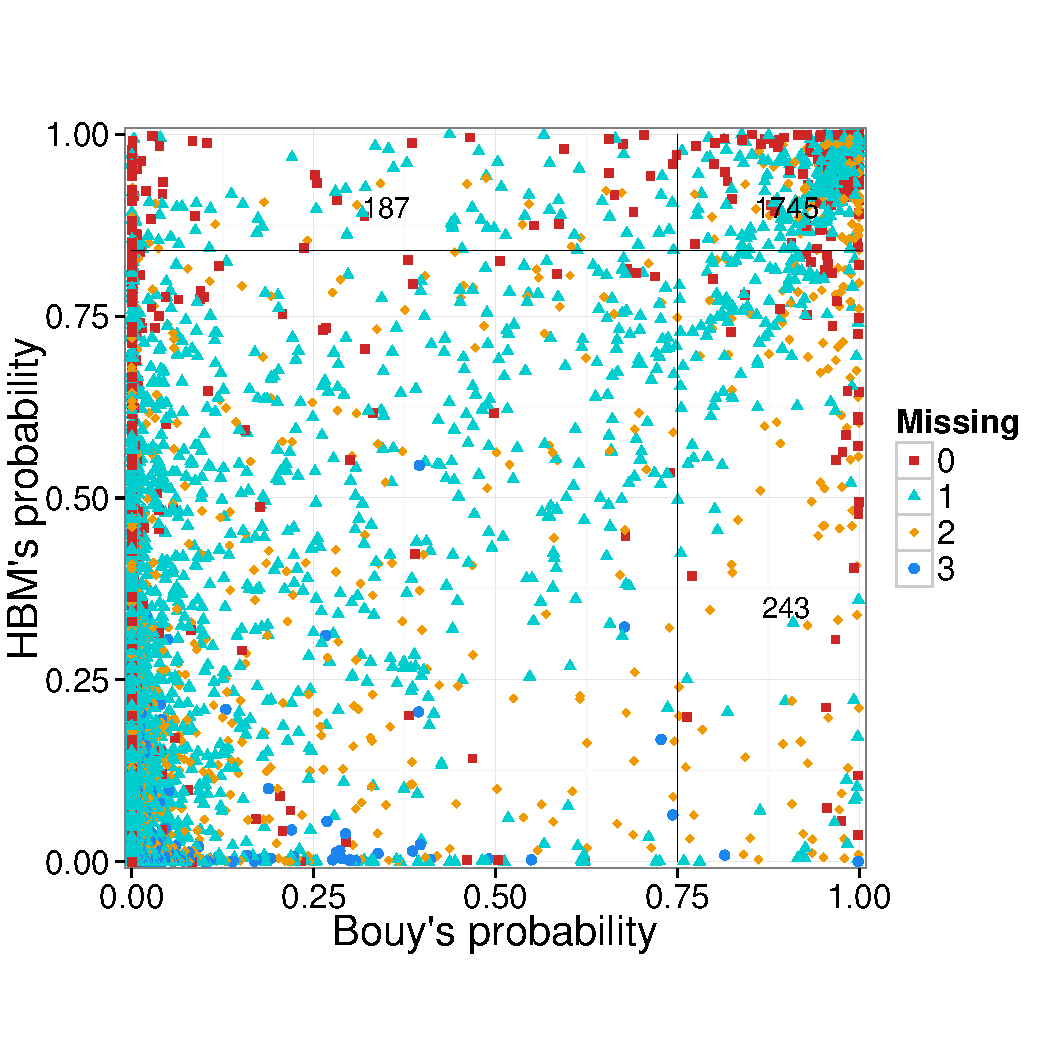
\includegraphics{figs/HBMvsBouy.pdf}}
\caption{Recovered membership probabilities compared to those of \citet{Bouy2015}. Lines show the 0.75 and $p_t=0.84$ probability thresholds used in both works. The numbers indicate the new candidate members (top left), rejected candidate members (bottom right), and common candidate members (top right).}
\label{figure:HM-SBB}
\end{center}
\end{figure}


 \begin{figure*}[htbp]
\begin{center}
%\resizebox{\hsize}{!}{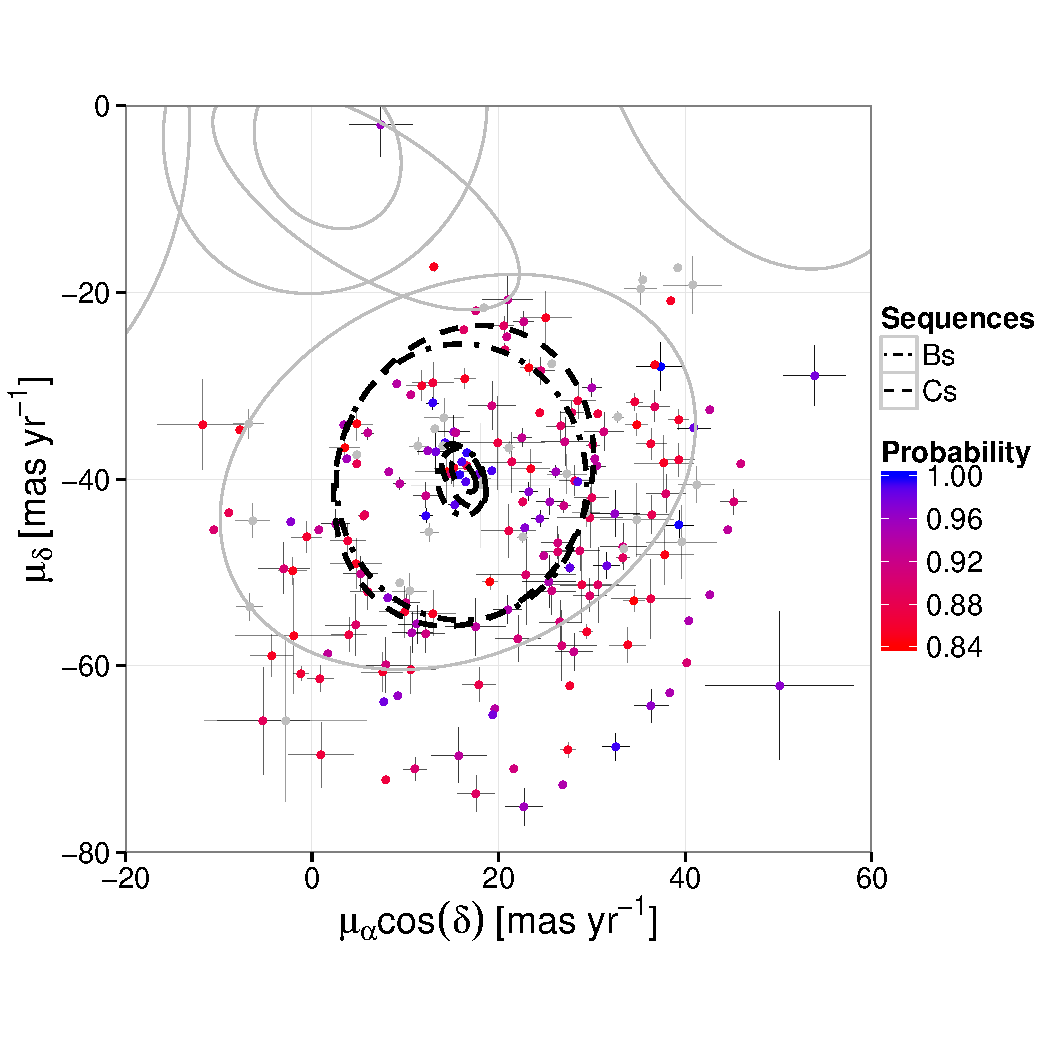
\includegraphics[page=1]{figs/NewOnes.pdf}\includegraphics[page=5]{figs/NewOnes.pdf}}
\caption{Proper motion (left) and $K_s$ vs. $i-K_s$ CMD (right) showing the new candidate members found in this work. Captions as in Fig. \ref{figure:probabilities}.}
\label{figure:newones}
\end{center}
\end{figure*}

 \begin{figure*}[htbp]
\begin{center}
%\resizebox{\hsize}{!}{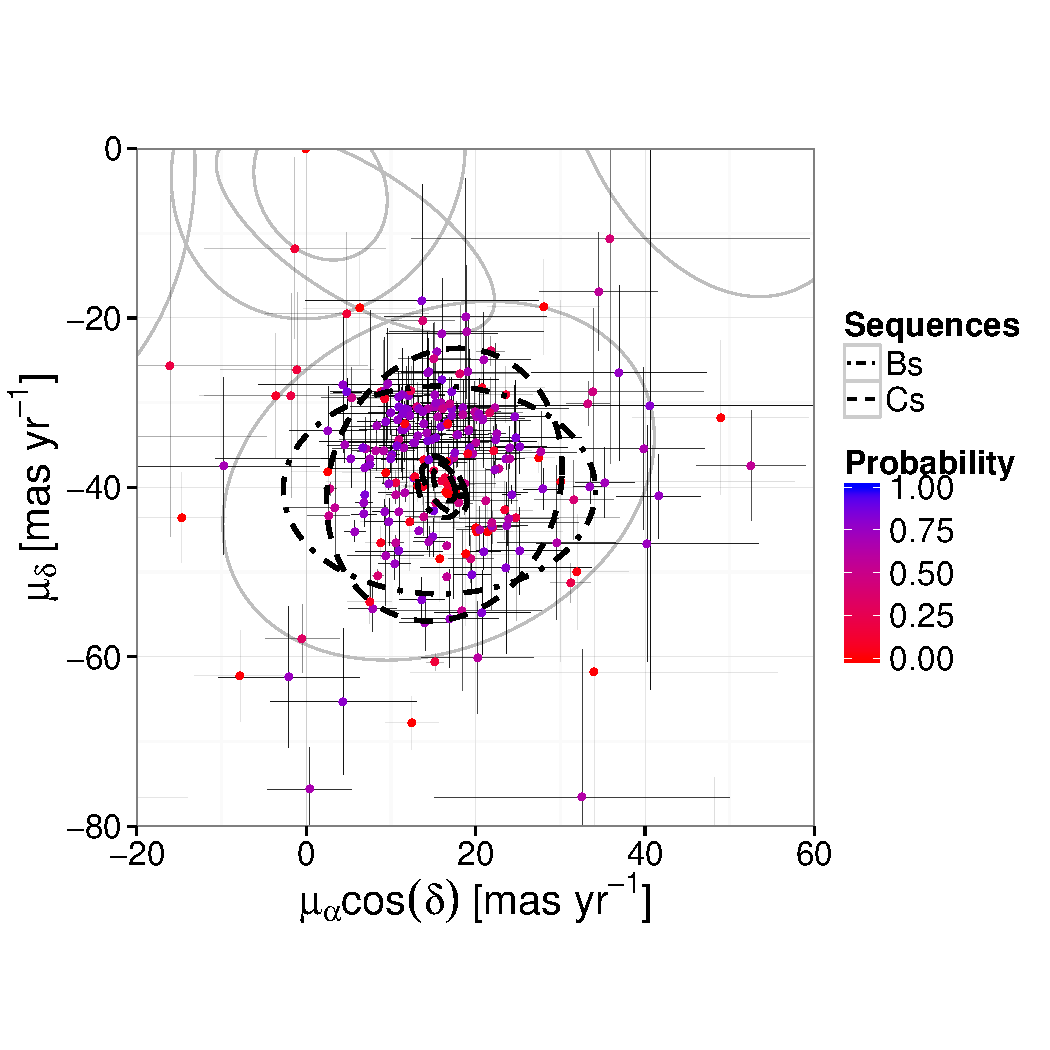
\includegraphics[page=1]{figs/Rejecteds.pdf}\includegraphics[page=5]{figs/Rejecteds.pdf}}
\caption{Proper motion (left) and $K_s$ vs. $i-K_s$ CMD (right) showing the rejected candidate members of \citet{Bouy2015}. Captions as in Fig. \ref{figure:probabilities}.}
\label{figure:rejecteds}
\end{center}
\end{figure*}

\begin{figure*}[htbp]
\begin{center}
%\resizebox{\hsize}{!}{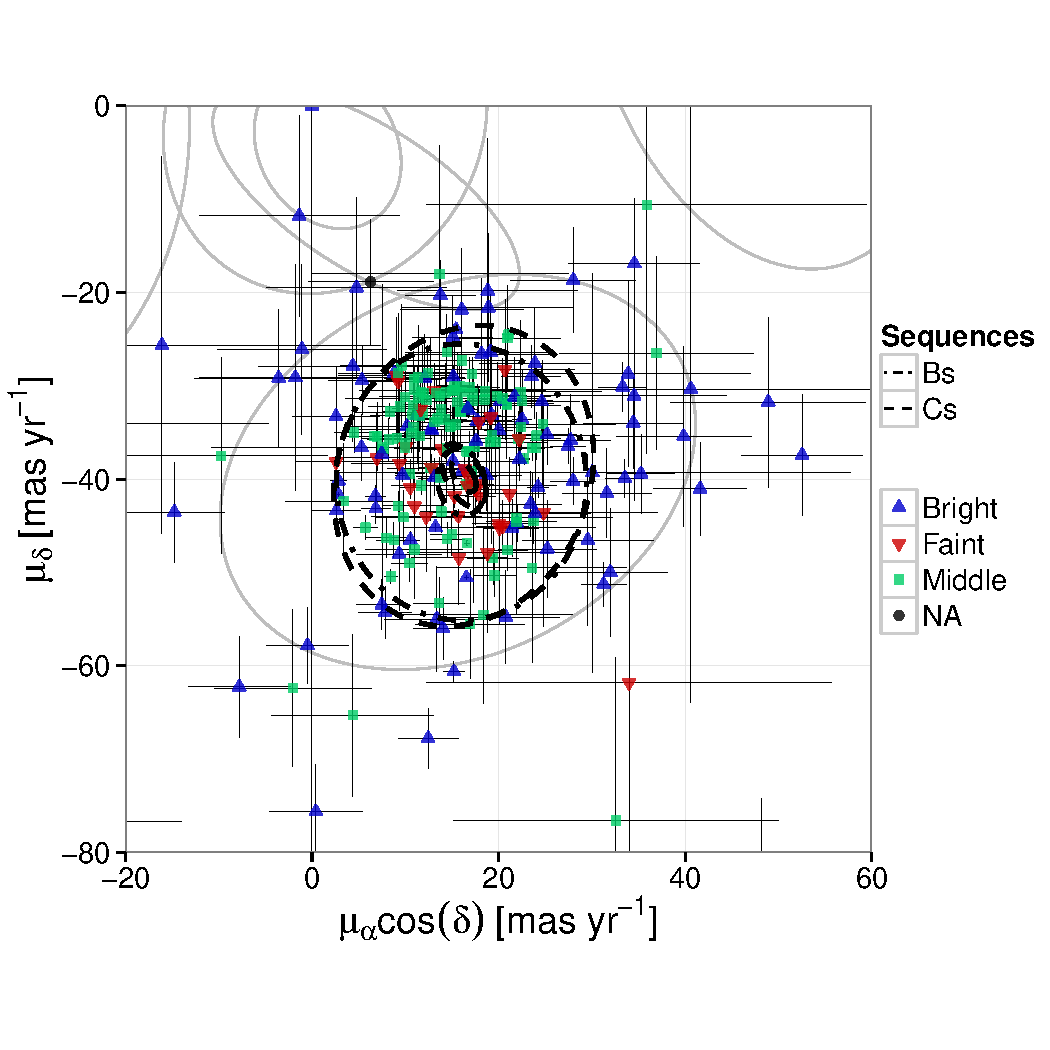
\includegraphics[page=1]{figs/RejectedsCOLORS.pdf}\includegraphics[page=5]{figs/RejectedsCOLORS.pdf}}
\caption{Proper motion (left) and $K_s$ vs. $i-K_s$ CMD (right) showing the rejected candidate members of \citet{Bouy2015}. The colours and shapes are a proxy for their $K_s$ magnitude.}
\label{figure:rejectedsCOLORS}
\end{center}
\end{figure*}
\subsubsection{Candidate members from \citet{Stauffer2007}}.
Here I would like to make a broad comparison of our list of members with that of Stauffer. I would do this for completeness.
The comparison must be done in terms of proper motions and photometry. If any other observable was taken into account the comparison is unfair. Nevertheless, this comparison is also important in the sense that the extra info can give some hints on possible improvements on the proper motions and photometric distributions
\section{Velocity distribution}
I must work on it. Here I must transform the bivariate proper motions distributions into a univariate velocity distributions using the distance and assuming spherical symmetry. This distribution will give us some hints to improve the proper motions model. It will be interesting to fit a model, maxwellian for example and see how well it fits. If more models are available we can try to find the best one in terms of Bayesian model selection. 
\section{Spatial distribution}
To include
\section{Luminosity distribution}
This Section describes the process by which the apparent $J,H$, and $K_s$ magnitudes distributions are obtained and then transformed into the absolute magnitude distribution. Later, I present  these distributions and compare them with those found by \citet{Bouy2015} and by us using only the objects with large membership probability. 

\subsection{Derivation of the magnitude distributions}
\label{subsect:deriveluminosity}
To derive the $J,H,K_s$ magnitude distributions I start with the colour index, $CI$, distribution. These distribution is a GMM whose parameters are inferred in the model. Since we also model the EMB, their fraction and photometric sequence are taken into accaount. We exemplify this derivation on the $K_s$ band, but similar transformations apply to the rest of the bands. 

To obtain the distribution of $K_s$ for the cluster objects, we introduce the colour index $CI$ as a nuisance parameter and then we marginalise it. Thus, 

\begin{align}
p(K_s | \boldsymbol{\theta}_c) & = \int p(K_s,CI | \boldsymbol{\theta}_c) \cdot dCI =  \int p(K_s | CI ,\boldsymbol{\theta}_c) \cdot p(CI|\boldsymbol{\theta}_c)\cdot dCI. \nonumber
\end{align}
The term $p(K_s | CI ,\boldsymbol{\theta}_c)$ corresponds to the GMM modelling the distribution of $CI$ (Eq. \ref{eq:colordist}), while $p(K_s | CI ,\boldsymbol{\theta}_c)$ is the probability of $K_s$ given the $CI$ and the cluster parameters $\boldsymbol{\theta}_c$. Since our photometric model takes into account the equal-mass binaries, we include them proportionally to their fraction, ($1-\pi_{CB}$). Thus,

\begin{align}
p(K_s | \boldsymbol{\theta}_c) & =  \int \left[\pi_{CB}\cdot p_{Cs}(K_s| CI, \boldsymbol{\theta}_c) + (1-\pi_{CB})\cdot p_{Bs}(K_s| CI, \boldsymbol{\theta}_c)\right]\nonumber \\& \cdot p_{CI}(CI|\boldsymbol{\theta}_c)\cdot dCI. \nonumber \\
& =   \pi_{CB} \int p_{Cs}(K_s| CI, \boldsymbol{\theta}_c) \cdot p_{CI}(CI|\boldsymbol{\theta}_c) dCI \nonumber \\
&+ (1-\pi_{CB})\int p_{Bs}(K_s| CI, \boldsymbol{\theta}_c) \cdot p_{CI}(CI|\boldsymbol{\theta}_c)\cdot  dCI. \nonumber \\
\end{align}

In this equation, $Cs$ and $Bs$ stand for cluster and equal-mass binaries sequences, respectively. The terms inside the integrals correspond to Equations \ref{eq:lik-seq} and \ref{eq:colordist}. However, since here we focus only on the distribution of $K_s$, we marginalise the rest of the bands. Also, we change the integration limits to those of the truncated colour distribution ($CI_{min}=0.8, CI_{max}=8$). Finally, we obtain

\begin{align}
&p(K_s | \boldsymbol{\theta}_c)  =   \pi_{CB} \int_{CI_{min}}^{CI_{max}}\left[ \left[\sum_{i=1}^5 \pi_{CI,i} \cdot \mathcal{N}_t(CI| \mu_{CI,i},\sigma_{CI,i})\right]\right. \nonumber \\
&\cdot  \left.\int_{\tilde{Y},\tilde{J},\tilde{H}}\mathcal{N}(\{CI,\tilde{Y},\tilde{J},\tilde{H},K_s\}|\boldsymbol{\mathcal{S}}(CI, \boldsymbol{\beta}),\Sigma_{clus})~d\tilde{Y}~d\tilde{J}~d\tilde{H}\right] \cdot dCI \nonumber \\
& + (1-\pi_{CB}) \int_{CI_{min}}^{CI_{max}}\left[\left[\sum_{i=1}^5 \pi_{CI,i} \cdot \mathcal{N}_t(CI| \mu_{CI,i},\sigma_{CI,i})\right]\right.\nonumber\\
&\cdot \left. \int_{\tilde{Y},\tilde{J},\tilde{H}}\mathcal{N}(\{CI,\tilde{Y},\tilde{J},\tilde{H},K_s\}|T_{Bs}(\boldsymbol{\mathcal{S}}(CI, \boldsymbol{\beta})),\Sigma_{clus})~d\tilde{Y}~d\tilde{J}~d\tilde{H}\right]\cdot dCI. \nonumber 
\end{align}

The derivation of the $J$ and $H$ magnitude distributions is similar to the procedure described for $K_s$. We notice that, the derivation of these magnitude distributions takes into account the equal mass binaries and the systems which could have different mass ratios. Therefore, these distributions correspond to those of the systems. 

Then, we obtain the luminosity distributions using the magnitude distributions, the parallax and extinction of the cluster. We assume that the parallax is normally distributed with mean, 7.44 mas, and standard deviation 0.42 mas \citep{Galli2017}. This parallax distribution is convolved with the magnitude distributions to obtain the absolute magnitude distributions. Finally, we deredenned them employing the canonical value, $A_v=0.12$ \citep{Guthrie1987}, which we transform to the $J,H,K_s$ values using the extinction law of \citet{Cardelli1989}.

Since our methodology prescribes the \emph{true} photometric quantities based on the \emph{true} colour index $CI$, therefore, the completeness limits of this $CI$ dictate those of the photometric bands. The upper completeness limits that \citet{Bouy2015} estimate for $i$ and $K_s$ are $i\approx23$ mag and $K_s\approx18$ mag (see their appendix A). As they also mention, due to the heterogeneous origins of the DANCe DR2 survey, its completeness is not homogeneous over its entire area. To overcome this issue, they identified a region, the inner three degrees of the cluster, with homogeneous spatial and depth coverage and restricted their sample to it. Here, instead of restricting the sample, we assume that the UKIDSS survey provides the homogeneous spatial coverage at the faint magnitudes, and quote more conservative completeness limits at the bright end. Figure \ref{figure:completeness} shows the $K_s$ and $i$ density  for all sources in the Pleiades DANCe DR2. The upper completeness limits correspond to the point with maximum density, $i=21.4$ mag, $K_s=18.1$ mag. For the lower completeness limits we choose $i=13.2$ mag and $K_s=11.0$ mag because the density of brighter objects shows a sharp decline, probably due to saturation.
Thus, we define the $CI$ completeness interval as that of all the points, along the cluster sequence in the $K_s$ vs. $i-K_s$ CMD, for which $i$ and $K_s$ are bounded by their upper and lower completeness limits, respectively. This results on $2.7<i-K_s<5.6$ mag. With it and the cluster sequence, we derive the completeness intervals for the $J,H,K_s$. Finally, we transform these intervals to absolute magnitudes and deredden them. 
\begin{figure}[htbp]
\begin{center}
%\resizebox{\hsize}{!}{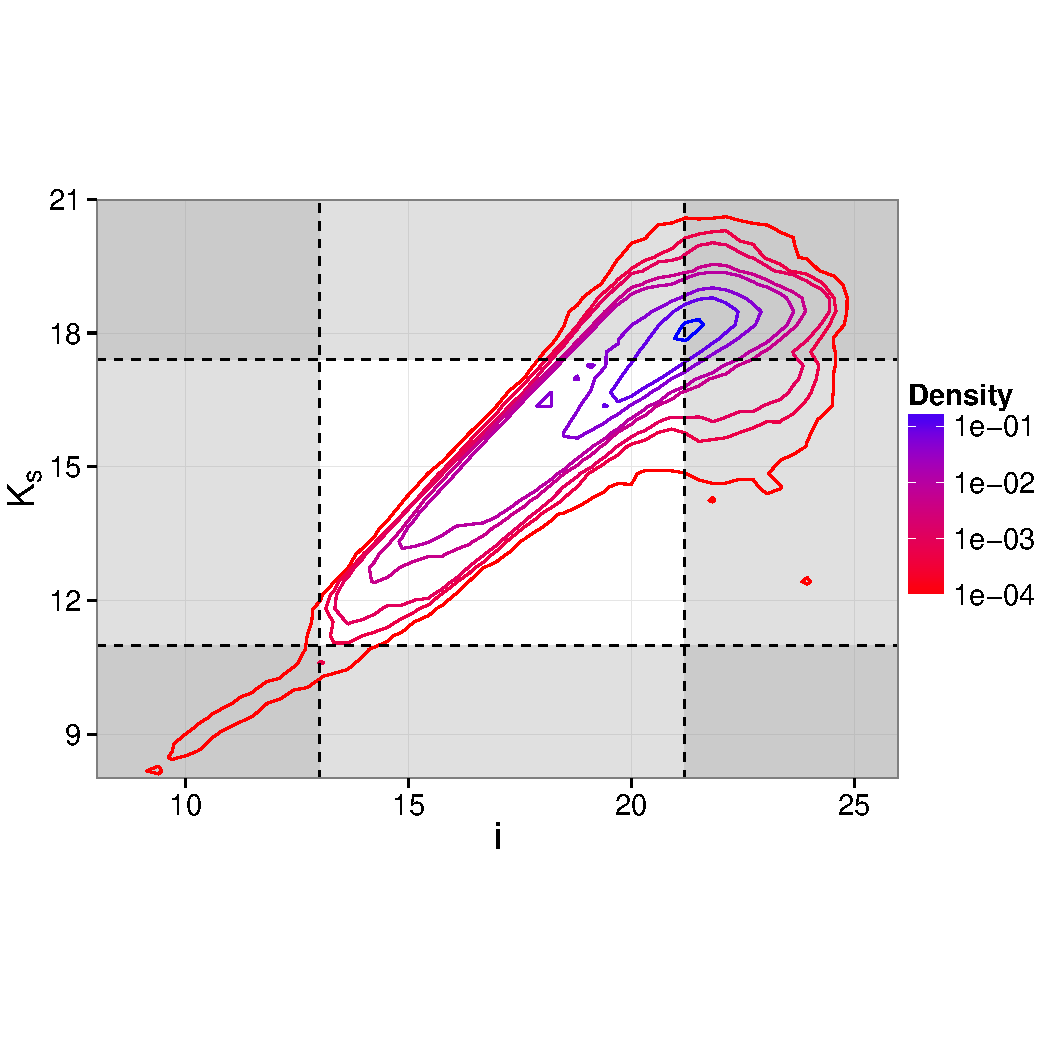
\includegraphics{figs/Density-Kvsi.pdf}}
\caption{Density of all DANCe DR2 sources in $K_s$ vs $i$ magnitudes. Lines show our completeness limits, $13.2<i<21.4$ mag and $11<K_s<18.1$ mag. The grey area is considered incomplete.}
\label{figure:completeness}.
\end{center}
\end{figure}


The luminosity distributions in $J,H,K_s$ together with their completeness limits are depicted (orange lines, hereafter continuous HBM-Hierarchical Bayesian Model) in Fig. \ref{figure:Luminosities}. For the sake of comparison we also show the luminosity distributions of: i) our candidate members ($p>p_t$) (black dashed line, hereafter discrete HBM), and, ii) the candidate members of \citet{Bouy2015} (blue dot-dashed line). We impute the missing values of the discrete cases using the nearest euclidean neighbour. The difference between the continuous HBM function and the discrete HBM comes from the imputed missing values and the objects used to obtain them. The continuous one uses all objects proportionally to their cluster membership probability while the discrete HBM uses only the high probability candidate members ($p>p_t$). We expect differences since the discrete HBM is not a random sample of the continuous HBM, therefore their distributions are not exactly alike. The differences between the discrete HBM and that of \citet{Bouy2015} arise mainly at the bright and faint end ($K_s\approx 4$ mag and $K_s\approx11$ mag). We argue that the origin of these differences lay in our new candidate members and the rejected ones of \citet{Bouy2015} (as discussed in Sect. \ref{sect:discussion}).

\begin{figure}[htbp]
\begin{center}
%\resizebox{\hsize}{!}{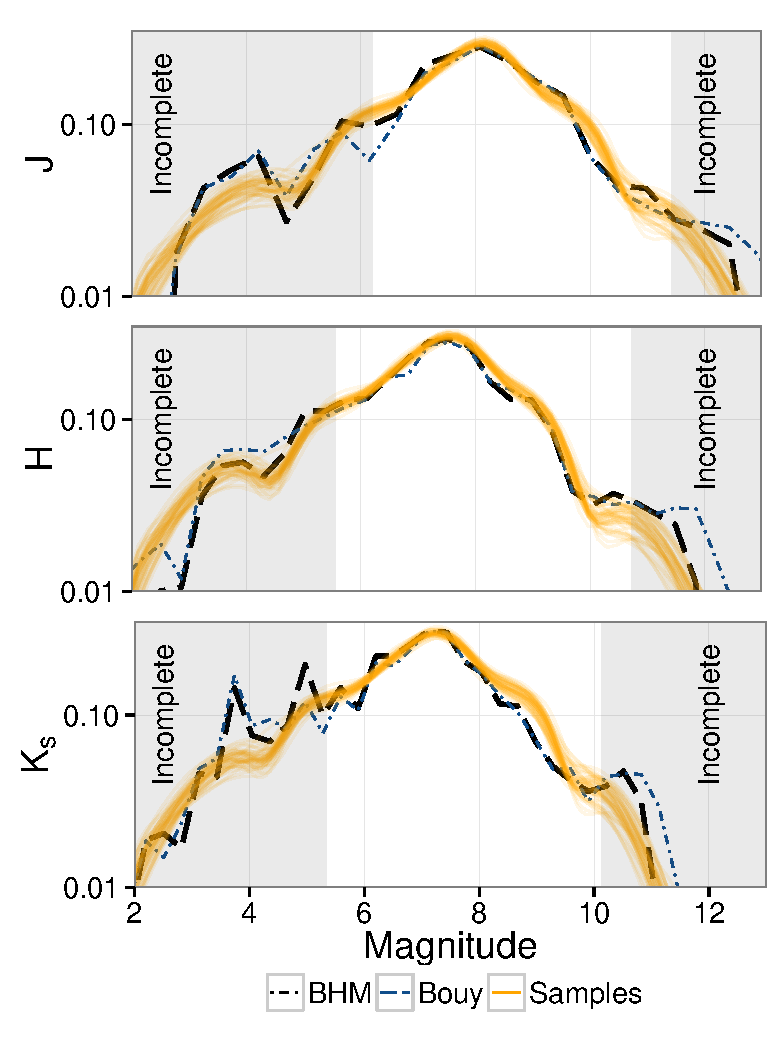
\includegraphics{figs/absolute_JHK-log.pdf}}
\caption{Luminosity functions from $J,H,K_s$ (orange). Also shown the regions of incompleteness and the luminosity functions computed from: the candidate members of \citet{Bouy2015} (dot-dashed blue line), and our candidate members, ($p_{84\%}>p_t$, dashed black line).}
\label{figure:Luminosities}.
\end{center}
\end{figure}

\section{Mass distribution}
\subsection{The mass-luminosity relation}
\subsection{Present day mass function}

Now, we proceed to compare the photometric distributions of the cluster population to those present in the literature. 
First, we compute the present day system mass function (PDSMF) and compare it to the Initial Mass Functions (IMF) of \citet{Chabrier2005} and \citet{Thies2007}. Then, we analyse and discuss the differences between the Pleiades PDSMF and those of the Trapezium and Hyades clusters. 

We obtain the PDSMF, independently in the $J,H,K_s$ bands, by transforming the luminosity functions into system mass functions using the mass-luminosity relations given by the BT-Settl models of \citet{Allard2012} (grid CIFIST2011bc for the 2MASS AB photometric system). Since the luminosity functions of Sect. \ref{subsubsect:luminosity} correspond to the luminosity of systems (single and binary stars), therefore the derived mass function is the system mass function. We assume an age of 120 Myr for the Pleiades together with solar metallicity. The transformation from luminosities to masses is proportional to the derivative of the mass-luminosity relation, and indeed very sensitive to it \cite[see][ for some words of caution]{DAntona1998}. Therefore, we decide to fit the BT-Settl grid with splines, and obtain the derivatives from this fit. 

Figure \ref{fig:MassFunction} shows the logarithmic PDSMF ($\xi_L$) for the $J,H,K_s$ bands normalised on the completeness limits of the survey (see Sect. \ref{subsubsect:luminosity}). This figure also shows, the PDSMF proposed by  \citet{Bouy2015} (blue dashed line) and, the IMFs of \citet{Thies2007} and \citet{Chabrier2005}. For this last one, we show its standard uncertainty \cite[taken from][]{Chabrier2003} as a sample of blue lines. As shown in this Fig., the PDSMFs of this work compare well with each others, and, in the overlap interval, with the one proposed by \citet{Bouy2015}. However, the difference that these PDSMFs show above $0.3 M_{\odot} (-0.5 < \log M/M_{\odot})$ may have its origin on the new and rejected candidate members. Particularly the new candidate members which are preferentially M stars (with masses in the range $0.075 - 0.6 M_{\odot}$ or $-1.12 < \log M/M_{\odot} < -0.22$). Also, similarly to what \citet{Bouy2015} pointed out, there is a possible flattening in the PDSMF below $50 M_{Jup}$ ($\log M/M_{\odot} < -1.3$). However, due to the level of uncertainty in this region we have not enough evidence to claim it.

Using \emph{PyMultiNest} \citep{Buchner2014}, we fit three models to our $K_s$ band PDSMF in the completeness interval: a log-normal distribution and two power-law distributions, $m^{-\alpha}$, with two and three segments. Table \ref{tab:fitPDSMF} show the parameters of these models together with their evidence. Judging by the evidence the best fit is the two segment power-law distribution (solid black line in Fig. \ref{fig:MassFunction}). This distributions is similar to that found by \citet{Bouy2015}, except for the flat part in the low-mass range and the less step slope in the high mass range. However, it is in clear discrepancy with the IMFs of \citet{Chabrier2005},  \cite[$m_c=0.25_{-0.016}^{+0.021}$ and $\sigma=0.55_{-0.01}^{+0.05}$, the uncertainties are those reported by][for single objects]{Chabrier2003} and of \citet{Thies2007}. The discrepancy between IMFs and PDSMFs may have its origin either on the not yet established uncertainties in the mass-luminosity relationships, on dynamical effects associated with age, or on both of them.

\begin{table*}[ht!]
\caption{Parameters and evidence of models fitted to the PDSMF}
\begin{center}
\begin{tabular}{lll}
Model&Parameters& Log Evidence\\
\hline
LogNormal&$m_c=0.36\pm0.03$&\\
                 &$\sigma=0.46\pm0.02$ & $18.1 \pm 0.1$\\
\hline
Two Segments &$\alpha_0=-0.11\pm0.06$ \ \ $m \in [0.04,0.22\pm0.01]$ & \\ 
&  $\alpha_1=1.13\pm0.1$ \ \ $m \in [0.22\pm0.01,0.56]$&$2222.7\pm0.4$\\
\hline
Three Segments &$\alpha_0=-0.05\pm0.6$ \ \ $m \in [0.04,0.08\pm0.03]$ & \\
                          &$\alpha_1=-0.1\pm0.1$ \ \ $m \in [0.08\pm0.03,0.22\pm0.01]$ & \\ 
                          &$\alpha_2=1.13\pm0.1$ \ \ $m \in [0.22\pm0.01,0.56]$&$2221.2\pm 0.3$\\
\hline
\end{tabular}
\end{center}
\label{tab:fitPDSMF}
\end{table*}%

Our PDSMF allows us to give a lower limit to the mass of the cluster. The mean mass of the cluster, in our entire mass range, is $0.26 \pm 0.006 M_{\odot}$. We compute the expected number of cluster members as the integral, over the whole range of membership probabilities, of number of objects at each membership probability, and its value is $3116 \pm 110$ objects. The product of the mean mass times the expected number of members is $807^{+38}_{-29} M_{\odot}$. Since we still lack the high mass range of the PDSMF, this value is a lower limit to the mass of the cluster. However, we can not claim further on our results. The quoted uncertainties are underestimated since they do not take into account the uncertainties in the mass-luminosity relations, which are yet to be established.

\begin{figure}[htbp]
\begin{center}
%\resizebox{\hsize}{!}{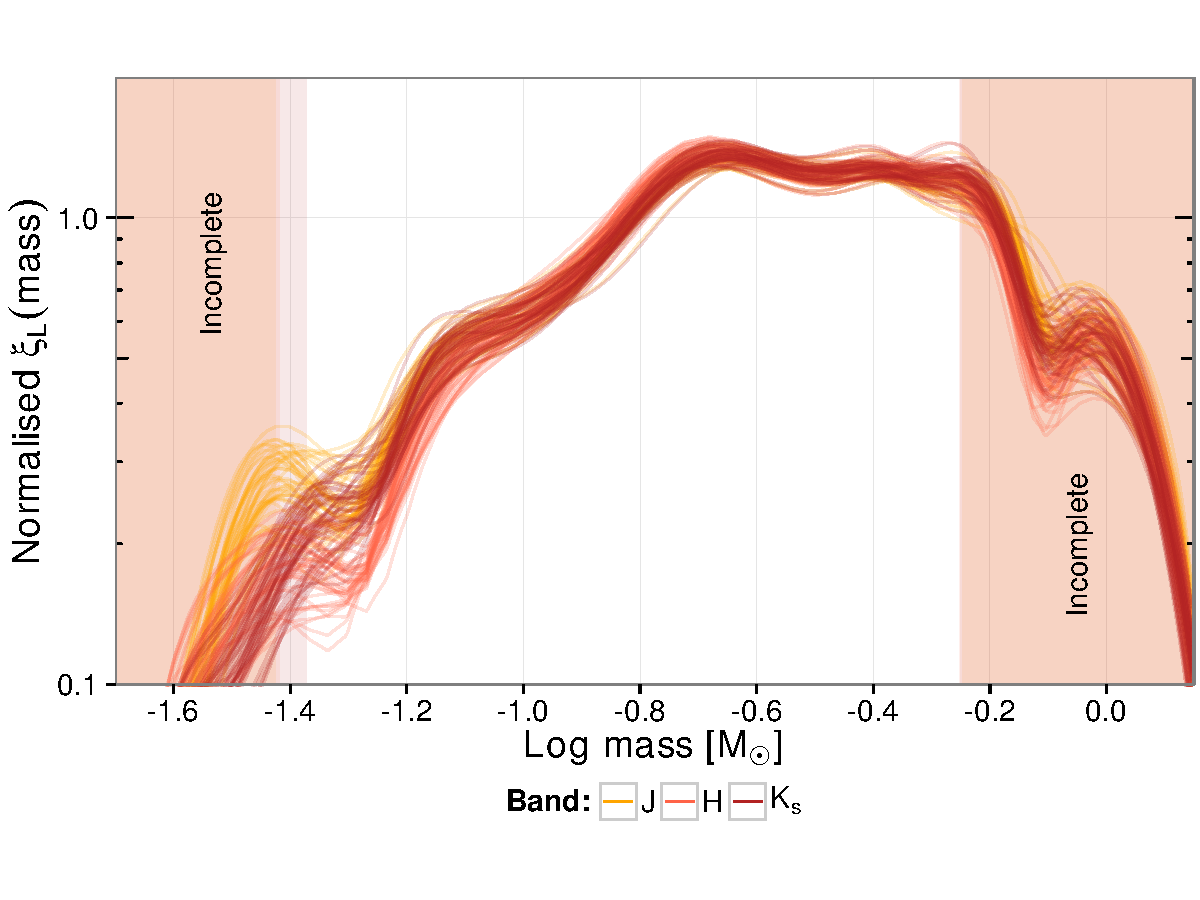
\includegraphics[page=1]{figs/MassDistribution.pdf}}
\caption{Normalised PDSMF in $J,H,K_s$ bands. Also shown the IMFs of \citet{Chabrier2005, Thies2007} and fits to the PDSMF found by us and \citet{Bouy2015}.}
\label{fig:MassFunction}.
\end{center}
\end{figure}

\section{The mass distribution on time}
Dynamical effects may have an impact on the cluster mass function. Figure \ref{fig:PDSMFcomparison} (left panel) compares the PDSMF from the Pleiades ($\approx120$ Myr) derived here, to those of the Trapezium ($\approx1$ Myr) and Hyades ($\approx 600$ Myr). These PDSMFs correspond to those of  Fig. 11 of \citet{Bouy2015} (private communication). As mentioned by \citet{Bouy2015}, the abundance of low-mass stars and brown dwarfs in the range $0.03 - 0.1 \ \ M_{\odot}$($\log M/M_{\odot} \approx \{-1, -1.4\}$) seems to diminish with time (since the PDSMF is normalised, this produces a relative increase of low-mass stars in the range $-0.4 < \log M/M_{\odot} < -0.2$). This effect is consistent with the classical scenario in which low-mass stars and brown dwarfs are ejected as the cluster relaxes. To test the validity of this scenario, at least the statistical significance of the observed differences among the PDSMF of this three clusters, we test the null hypothesis that the Trapezium and the Hyades have the same PDSMF as the Pleiades. Since we just have the cluster model of the Pleiades, we are not able to perform model comparison in a bayesian fashion. Thus, to do the statistical comparison of these three clusters PDSMF we use the Kolmogorov-Smirnov and Anderson-Darling tests. 

\begin{figure*}[htp]
\begin{center}
%\resizebox{\hsize}{!}{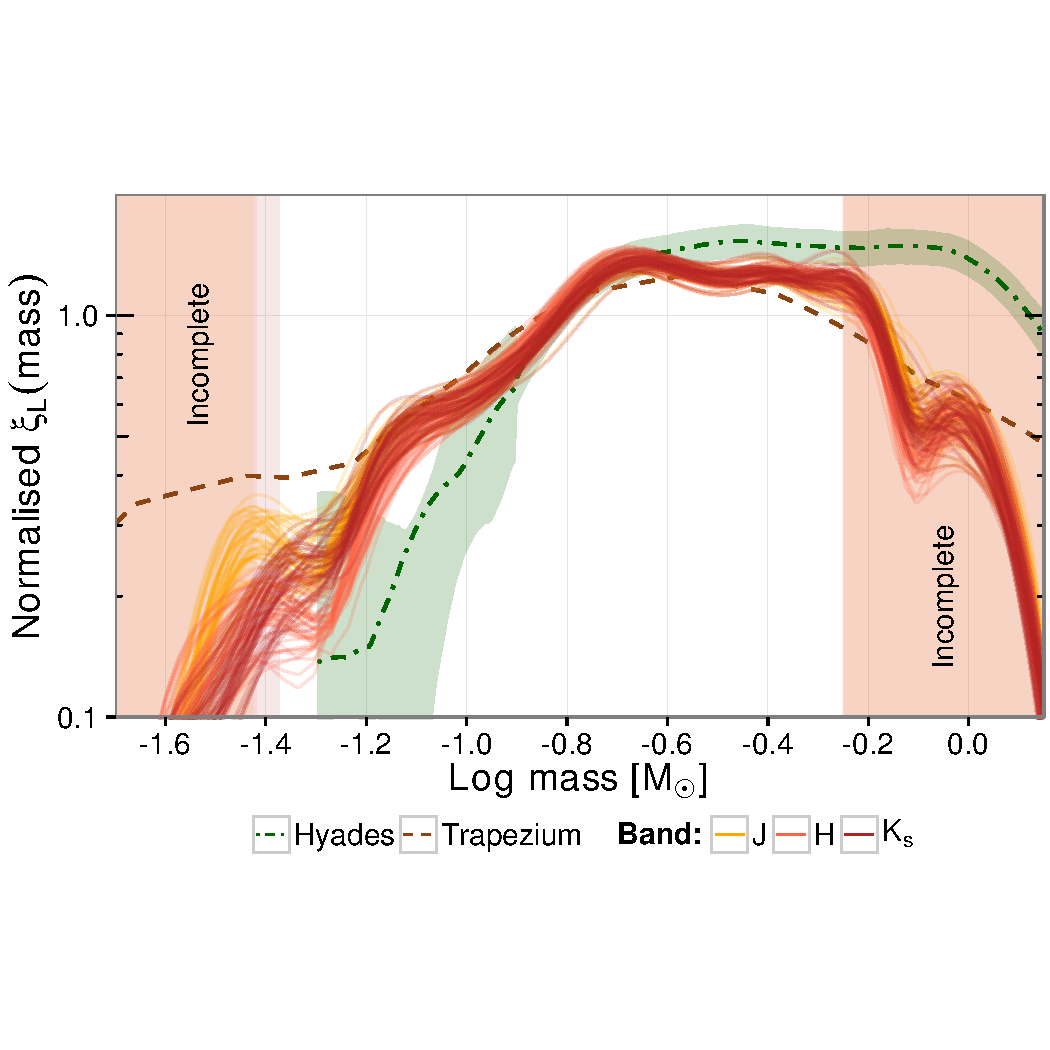
\includegraphics{figs/M45vsM42vsM44.pdf}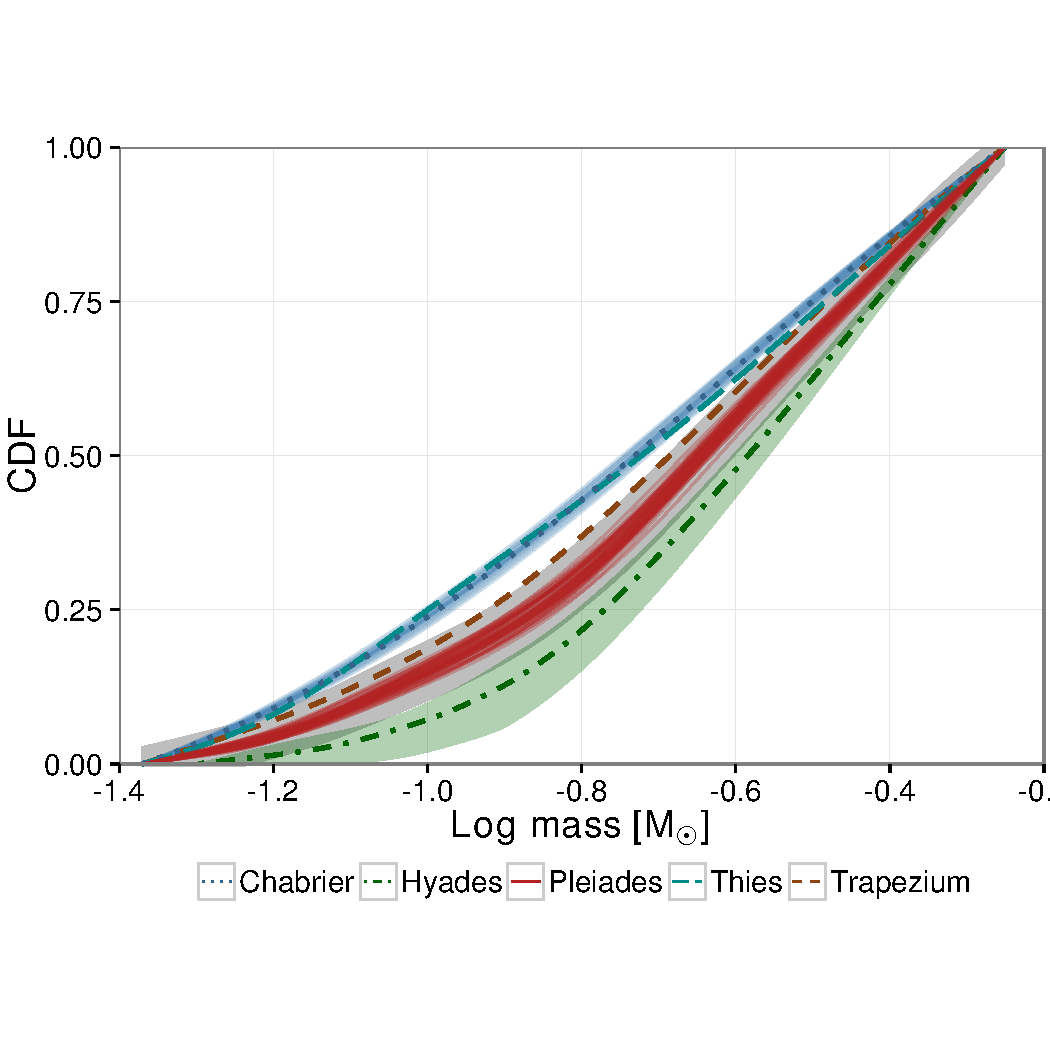
\includegraphics{figs/CDF_comparison.pdf}}
\caption{Left: PDSMFs of the Pleiades (derived here for $J,H,K_s$ bands), Trapezium, and Hyades, from \citet{Bouy2015}. They are normalised in the interval of completeness. Right: Cumulative distribution functions (CDF) of the PDSMFs from left panel and that of \citet{Chabrier2005} and \citet{Thies2007} system initial mass function (normalised also in the interval of completeness). The Pleiades CDF shown is just from $K_s$ band. The grey area depicts the area in which the null hypothesis of same PDSMF as that of the Pleiades can not be rejected (at $\alpha=0.01$).}
\label{fig:PDSMFcomparison}.
\end{center}
\end{figure*}


The right panel of Fig. \ref{fig:PDSMFcomparison} shows the cumulative distribution functions (CDFs) of  the Trapezium, Pleiades (only in $K_s$ band) and Hyades PDSMFs. Also and for comparison,  we show the CDFs of \citet{Chabrier2005} and \citet{Thies2007} IMFs. The grey area around the Pleiades CDF shows the hypothesis test in which we compare each CDF with that of the Pleiades. The null hypothesis is that each compared CDF is exactly that of the Pleiades. We use the Kolmogorov-Smirnov statistic and the alpha value $\alpha = 0.01$, to compute the vertical distance $d_{\alpha}$ from the Pleiades CDF, the grey region. The null hypothesis is rejected only if the tested CDF lies entirely outside the grey region around the Pleiades CDF. As can be seen, neither the IMFs nor the PDSMF of the Trapezium and Hyades lay entirely within the grey area, thus we can reject the null hypothesis that they share the same PDSMF of the Pleiades. Furthermore, since the Kolmogorov-Smirnov test uses only the maximum distance between CDFs, we also applied the more robust Anderson-Darling test. It also rejects the null hypotheses (at $p < 0.004$) that the Trapezium and Hyades PDSMFs and the \citet{Chabrier2005} and \citet{Thies2007} IMFs have the same CDF of the Pleiades. 

The previous tests show that there is enough evidence to claim for differences among the PDSMFs of these three clusters and from IMFs and Pleiades PDSMF. Thus suggesting that these differences may have an origin on dynamical effects associated with age and relaxation. Nevertheless, to claim for reliable evidence supporting these differences the census of the Trapezium and Hyades must be done using the same methods. Also, the uncertainties must be properly establish both for the other PDSMFs and for the mass-luminosity relation from which all these PDSMF are derived. 

\section{Updating the previous knowledge}
